\subsection{Slučaj upotrebe: Predaja materijala}

\subsubsection*{Kratak opis:}

Član produkcionog tima započinje rad na dodeljenom zadatku i predaje završen materijal, nakon čega zadatak prelazi na pregled kod Projektnog menadžera.

\subsubsection*{Akteri:}
\begin{itemize}
	\item \textbf{Član produkcionog tima} -- apstraktni akter koji kreira materijale opisan u poglavlju \textbf{Akteri}.
\end{itemize}

\subsubsection*{Preduslovi:}
\begin{itemize}
	\item Član tima je prijavljen na sistem.
	\item Član tima ima dodeljen zadatak u statusu „Dodeljen“, „U Radu“ ili „Za Doradu“.
	\item Sistem je ispravan.
\end{itemize}

\subsubsection*{Postuslovi:}
\begin{itemize}
	\item Materijal je sačuvan u sistemu i povezan je sa zadatkom.
	\item Status zadatka je „Predat Na Pregled“.
	\item Projektni menadžer je obavešten o predaji materijala.
\end{itemize}

\subsubsection*{Osnovni tok:}
\begin{enumerate}
	\item Član tima bira opciju „Moji Zadaci“.
	\item Sistem prikazuje listu zadataka dodeljenih članu tima.
	\item Član tima bira zadatak.
	\item Sistem prikazuje detalje zadatka (opis, rok, status, ranije predate verzije ukoliko postoje).
	\begin{itemize}
		\item Ukoliko je zadatak u statusu „Za Doradu“, izvršava se podtok P1, a zatim podtok P2.
		\item Ukoliko zadatak nije u statusu „U Radu“, izvršava se podtok P2.
	\end{itemize}
	\item Član tima bira opciju „Predaj Materijal“.
	\item Sistem prikazuje formu za predaju materijala.
	\item Član tima unosi podatke o materijalu i otprema fajl.
	\item Član tima potvrđuje predaju.
	\item Sistem proverava ispravnost podataka i fajla i da li je zadatak još uvek aktivan.
	\item Sistem čuva materijal kao novu verziju i povezuje ga sa zadatkom.
	\item Sistem automatski menja status zadatka u „Predat Na Pregled“.
	\item Sistem obaveštava Projektnog menadžera.
	\item Sistem prikazuje potvrdu o uspešnoj predaji.
\end{enumerate}

\subsubsection*{Podtokovi:}

\paragraph*{P1: Pregled komentara pri doradi}
\begin{enumerate}
	\item Sistem prikazuje komentare Projektnog menadžera i prethodno predatu verziju.
	\item Član tima pregleda komentare.
\end{enumerate}

\paragraph*{P2: Započinjanje rada}
\begin{enumerate}
	\item Član tima bira opciju „Započni Rad“.
	\item Sistem menja status zadatka u „U Radu“ i beleži vreme početka rada.
	\item Nastavlja se od koraka 5 osnovnog toka.
\end{enumerate}

\subsubsection*{Alternativni tokovi:}

\paragraph*{A1: Neispravni podaci ili fajl}
\begin{itemize}
	\item Ovaj tok se dešava u koraku 9 ukoliko obavezna polja nisu popunjena, uneti podaci nisu ispravni, format fajla nije podržan ili je prekoračena dozvoljena veličina fajla.
	\item Sistem prikazuje poruku o grešci i označava problem.
	\item Povratak na korak 7 osnovnog toka.
\end{itemize}

\paragraph*{A2: Neuspešno otpremanje fajla}
\begin{itemize}
	\item Ovaj tok se dešava u koraku 10 ukoliko dođe do prekida veze ili greške pri čuvanju.
	\item Sistem ne čuva materijal, ne menja status zadatka, zadržava unete podatke i prikazuje poruku o grešci.
	\item Povratak na korak 8 osnovnog toka.
\end{itemize}

\paragraph*{A3: Zadatak više nije aktivan}
\begin{itemize}
	\item Ovaj tok se dešava u koraku 9 ukoliko je zadatak u međuvremenu otkazan.
	\item Sistem odbija predaju i prikazuje poruku da zadatak više nije aktivan.
	\item Slučaj upotrebe se završava neuspešno.
\end{itemize}

\subsubsection*{Specijalni zahtevi:}
\begin{itemize}
	\item Sistem čuva sve verzije materijala i nikada ne briše prethodnu.
	\item Za svaku verziju se beleže autor i vreme predaje.
	\item Opcija „Predaj materijal“ dostupna je samo za zadatke u statusu „U Radu“.
	\item Član tima može istovremeno imati više zadataka u statusu „U Radu“. Slučaj upotrebe se izvršava zasebno za svaki zadatak, a predaja materijala može da usledi u bilo kom kasnijem izvršavanju.
	\item Pregled liste zadataka, detalja i komentara ne menja status zadatka. Statuse zadatka menja isključivo sistem, kao posledicu akcija korisnika.
	\item Dozvoljeni formati i najveća veličina fajla definišu se na nivou sistema.
\end{itemize}

\subsubsection*{Dodatne informacije:}
\begin{itemize}
	\item Polja forme uključuju:
	\begin{itemize}
		\item Tip materijala, naziv, napomenu i fajl (jedan ili više) unosi član tima.
		\item Zadatak, autor, datum, vreme i broj verzije popunjava sistem automatski.
	\end{itemize}
	\item Statusi zadatka i trenuci njihove promene:
	\begin{itemize}
		\item \textbf{Dodeljen}: Projektni menadžer kreira i dodeljuje zadatak.
		\item \textbf{U Radu}: Član tima izabere opciju „Započni rad“.
		\item \textbf{Predat Na Pregled}: Član tima preda materijal.
		\item \textbf{Za Doradu}: Projektni menadžer vrati materijal na doradu.
		\item \textbf{Završen}: Projektni menadžer odobri materijal.
	\end{itemize}
	\item Tipovi materijala po ulozi:
	\begin{itemize}
		\item \textbf{Storyboarder}: Skice kadrova.
		\item \textbf{Dizajner}: Dizajn likova, dizajn okruženja.
		\item \textbf{Animator}: Animirane sekvence, pojedinačni frejm animacije.
		\item \textbf{Audio dizajner}: Muzika, zvučni zapisi, zvučni efekti.
	\end{itemize}
\end{itemize}

\begin{figure}[H]
	\centering
	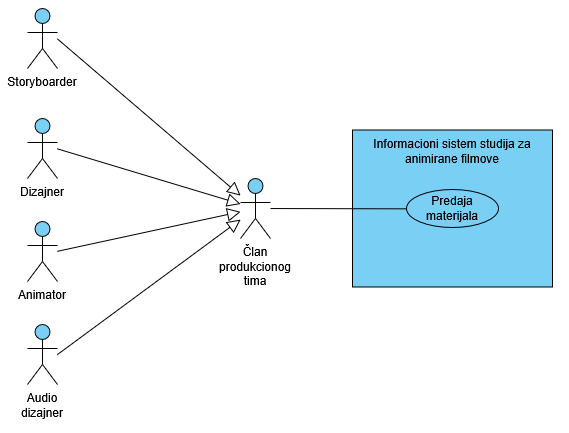
\includegraphics[width=\textwidth]{./dijagrami/dijagrami_slucajeva_upotrebe/slucaj_upotrebe_predaja_materijala.png} 
	\caption{Dijagram slučaja upotrebe ,,Predaja materijala''}
\end{figure}

\begin{figure}[H]
	\centering
	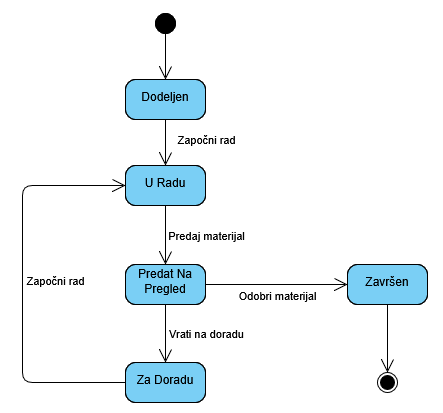
\includegraphics[width=\textwidth]{./dijagrami/dijagrami_stanja/dijagram_stanja_predaja_materijala.png} 
	\caption{Dijagram stanja ,,Predaja materijala''}
\end{figure}

\begin{figure}[H]
	\centering
	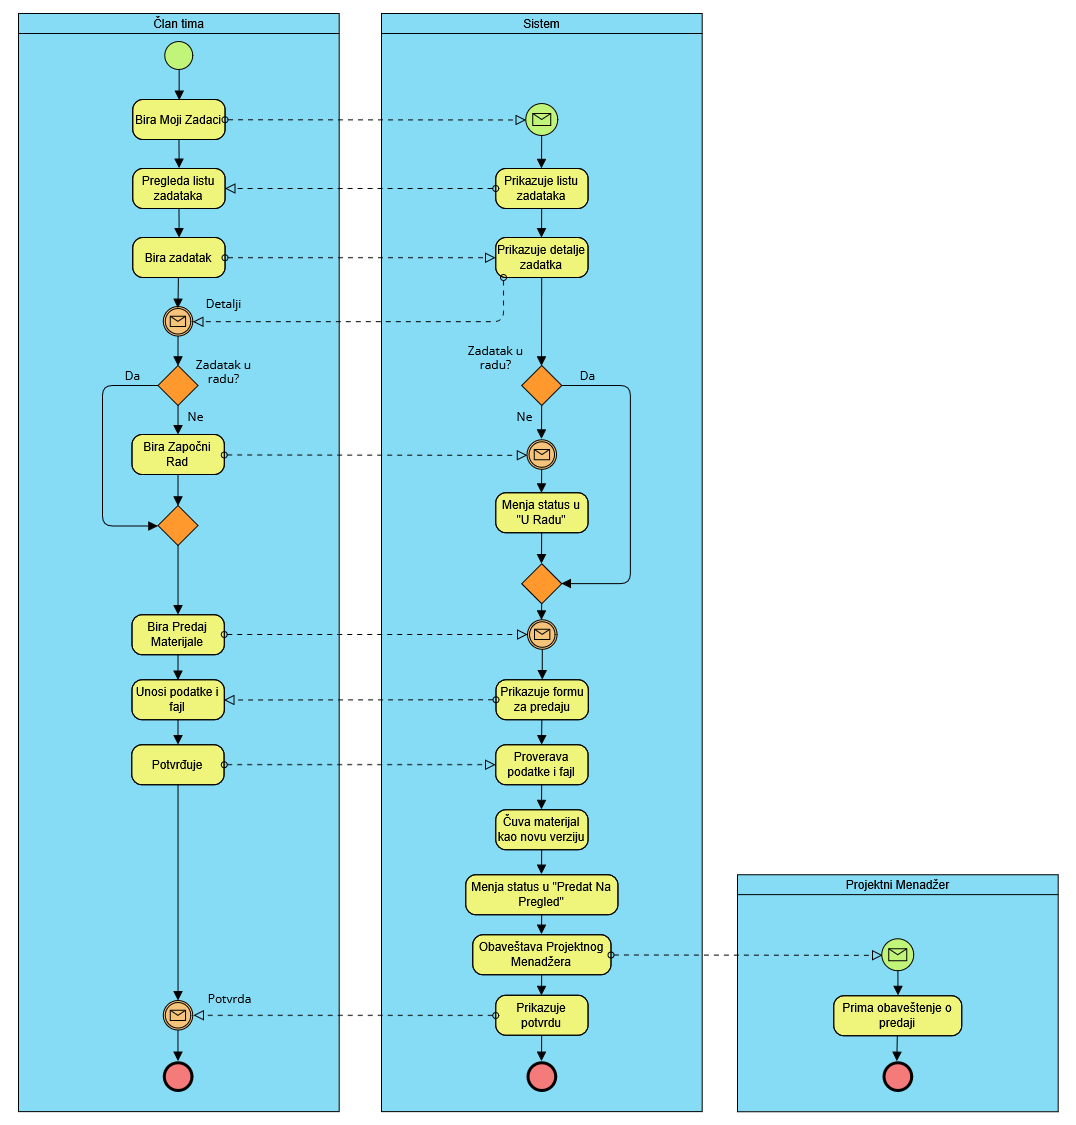
\includegraphics[width=\textwidth]{./dijagrami/bpmn/predaja_materijala.png} 
	\caption{BPMN dijagram saradnje ,,Predaja materijala''}
\end{figure}

\newpage